\documentclass[a0paper,portrait]{tikzposter}

\usepackage[utf8]{inputenc}
\usepackage[T1]{fontenc}
\usepackage{lmodern}
\usepackage{microtype}
\usepackage{amsmath,amssymb}
\usepackage{graphicx}
\usepackage{booktabs}
\usepackage{tabularx}
\usepackage{array}
\usepackage{xcolor}
\usepackage{enumitem}

\graphicspath{{results/presentation/}{results/}}
\setlist[itemize]{nosep,leftmargin=*}

\definecolor{DeepNavy}{HTML}{0B1F3A}
\definecolor{Photon}{HTML}{007C89}
\definecolor{Mist}{HTML}{EEF6F6}
\definecolor{Ink}{HTML}{1F2937}
\definecolor{Amber}{HTML}{D97706}

\definecolorpalette{posterpalette}{
    \definecolor{colorOne}{named}{DeepNavy}
    \definecolor{colorTwo}{named}{Photon}
    \definecolor{colorThree}{named}{Mist}
}
\usecolorpalette{posterpalette}
\usetheme{Simple}
\useblockstyle{Default}
\usetitlestyle{Filled}
\colorlet{blocktitlebgcolor}{DeepNavy}
\colorlet{blocktitlefgcolor}{white}
\colorlet{blockbodybgcolor}{white}
\colorlet{blockbodyfgcolor}{Ink}
\colorlet{backgroundcolor}{white}

\newcommand{\pjbit}{pJ/bit}
\newcommand{\tbps}{Tb/s}
\newcolumntype{Y}{>{\raggedright\arraybackslash}X}

\title{\parbox{0.94\linewidth}{\centering Topology-Aware Mapping for Photonic Interconnects \\ in TPU-Class LLM Accelerators}}
\author{Pranav Sitaraman \quad \textbullet \quad Simone Surdi}
\institute{MIT 6.5930 Hardware Architectures for Deep Learning \quad \textbullet \quad Project 12: Evaluate a New Technology}

\settitle{
\centering
{\bfseries\color{white}\Huge \@title}\vskip0.6ex
{\color{white}\Large \@author}\vskip0.3ex
{\color{white}\large \@institute}
}

\begin{document}
\maketitle

\begin{columns}
\column{0.47}
\block{1. Motivation}{\normalsize
TPU pods succeed not because each chip is faster in isolation but because thousands of chips are wired together with a carefully designed memory and interconnect system. The most recent TPU7x/Ironwood pods publicly expose 9216 chips per pod, 192~GiB of HBM per chip, and 1200~GB/s of bidirectional inter-chip bandwidth per chip. For language model training and inference at this scale, the hard part is moving things---decode caches, expert tokens, gradients, layer-tied weights---rather than computing them.

\medskip
\textbf{Question.} If a future TPU pod were wired with Lightmatter Passage-style photonic interconnect, would we just observe a lower-energy link, or would the optimal memory placement and distributed schedule above the link change as well?
}

\column{0.53}
\block{2. Underlying Principles}{\normalsize
\textbf{Four conceptual layers.} We separate the workload (an einsum), the architecture (per-chip memory plus a logical cluster-memory level), the inner mapping picked by the mapper, and the distributed schedule chosen above the mapper (point-to-point exchange, remote pooled-HBM streaming, replicated cache, photonic multicast cache fill).

\medskip
\textbf{Network model.}
\[
E_{\text{net}} = B\bigl(e_c + h\,\ell(N)\,e_{tx}\bigr),\quad
T_{\text{net}} = \frac{B}{BW/C(N)} + h\,t_r + h\,\ell(N)\,t_p + t_s.
\]
Electrical and chiplet links pay an energy term that grows with average path distance. Photonic links are conversion-dominated and stay nearly flat. Non-multicast baselines pay every receiver. Photonic multicast pays the unique payload exactly once.

\medskip
\textbf{Iterative loop.} The mapper runs, its traffic is priced through the topology, and the resulting energy and latency are folded back into the logical-memory level. The mapper is then rerun until those per-bit numbers stabilize.
}
\end{columns}

\begin{columns}
\column{0.47}
\block{3. Evaluation Setup}{\normalsize
\begin{itemize}
\item \textbf{Held fixed:} compute (MAC, register file, unified buffer) and per-chip HBM energy and latency.
\item \textbf{Varied:} interconnect technology, topology, multicast support, and the distributed schedule.
\item \textbf{Baselines:} an electrical TPU-style torus and a deliberately strong 3.5~\tbps{}, 6~\pjbit{} chiplet baseline so the comparison is not against straw electronics.
\item \textbf{Photonics:} EVK100 (3.2~\tbps{} class, 1.9--3.2~\pjbit{}) and M1000 (57.3~\tbps{} one-way, 2.3~\pjbit{} including laser, multicast-capable optical circuit switching).
\item \textbf{Workloads:} six representative GEMM proxies (decode MLP, KV attention, prefill projection, long-context prefill, mixture-of-experts dispatch, training weight gradient) plus public Gemma~4 anchors and an explicitly labeled long-context Gemini-class stress proxy.
\end{itemize}
}

\column{0.53}
\block{4. Final Experiment Spine}{\centering
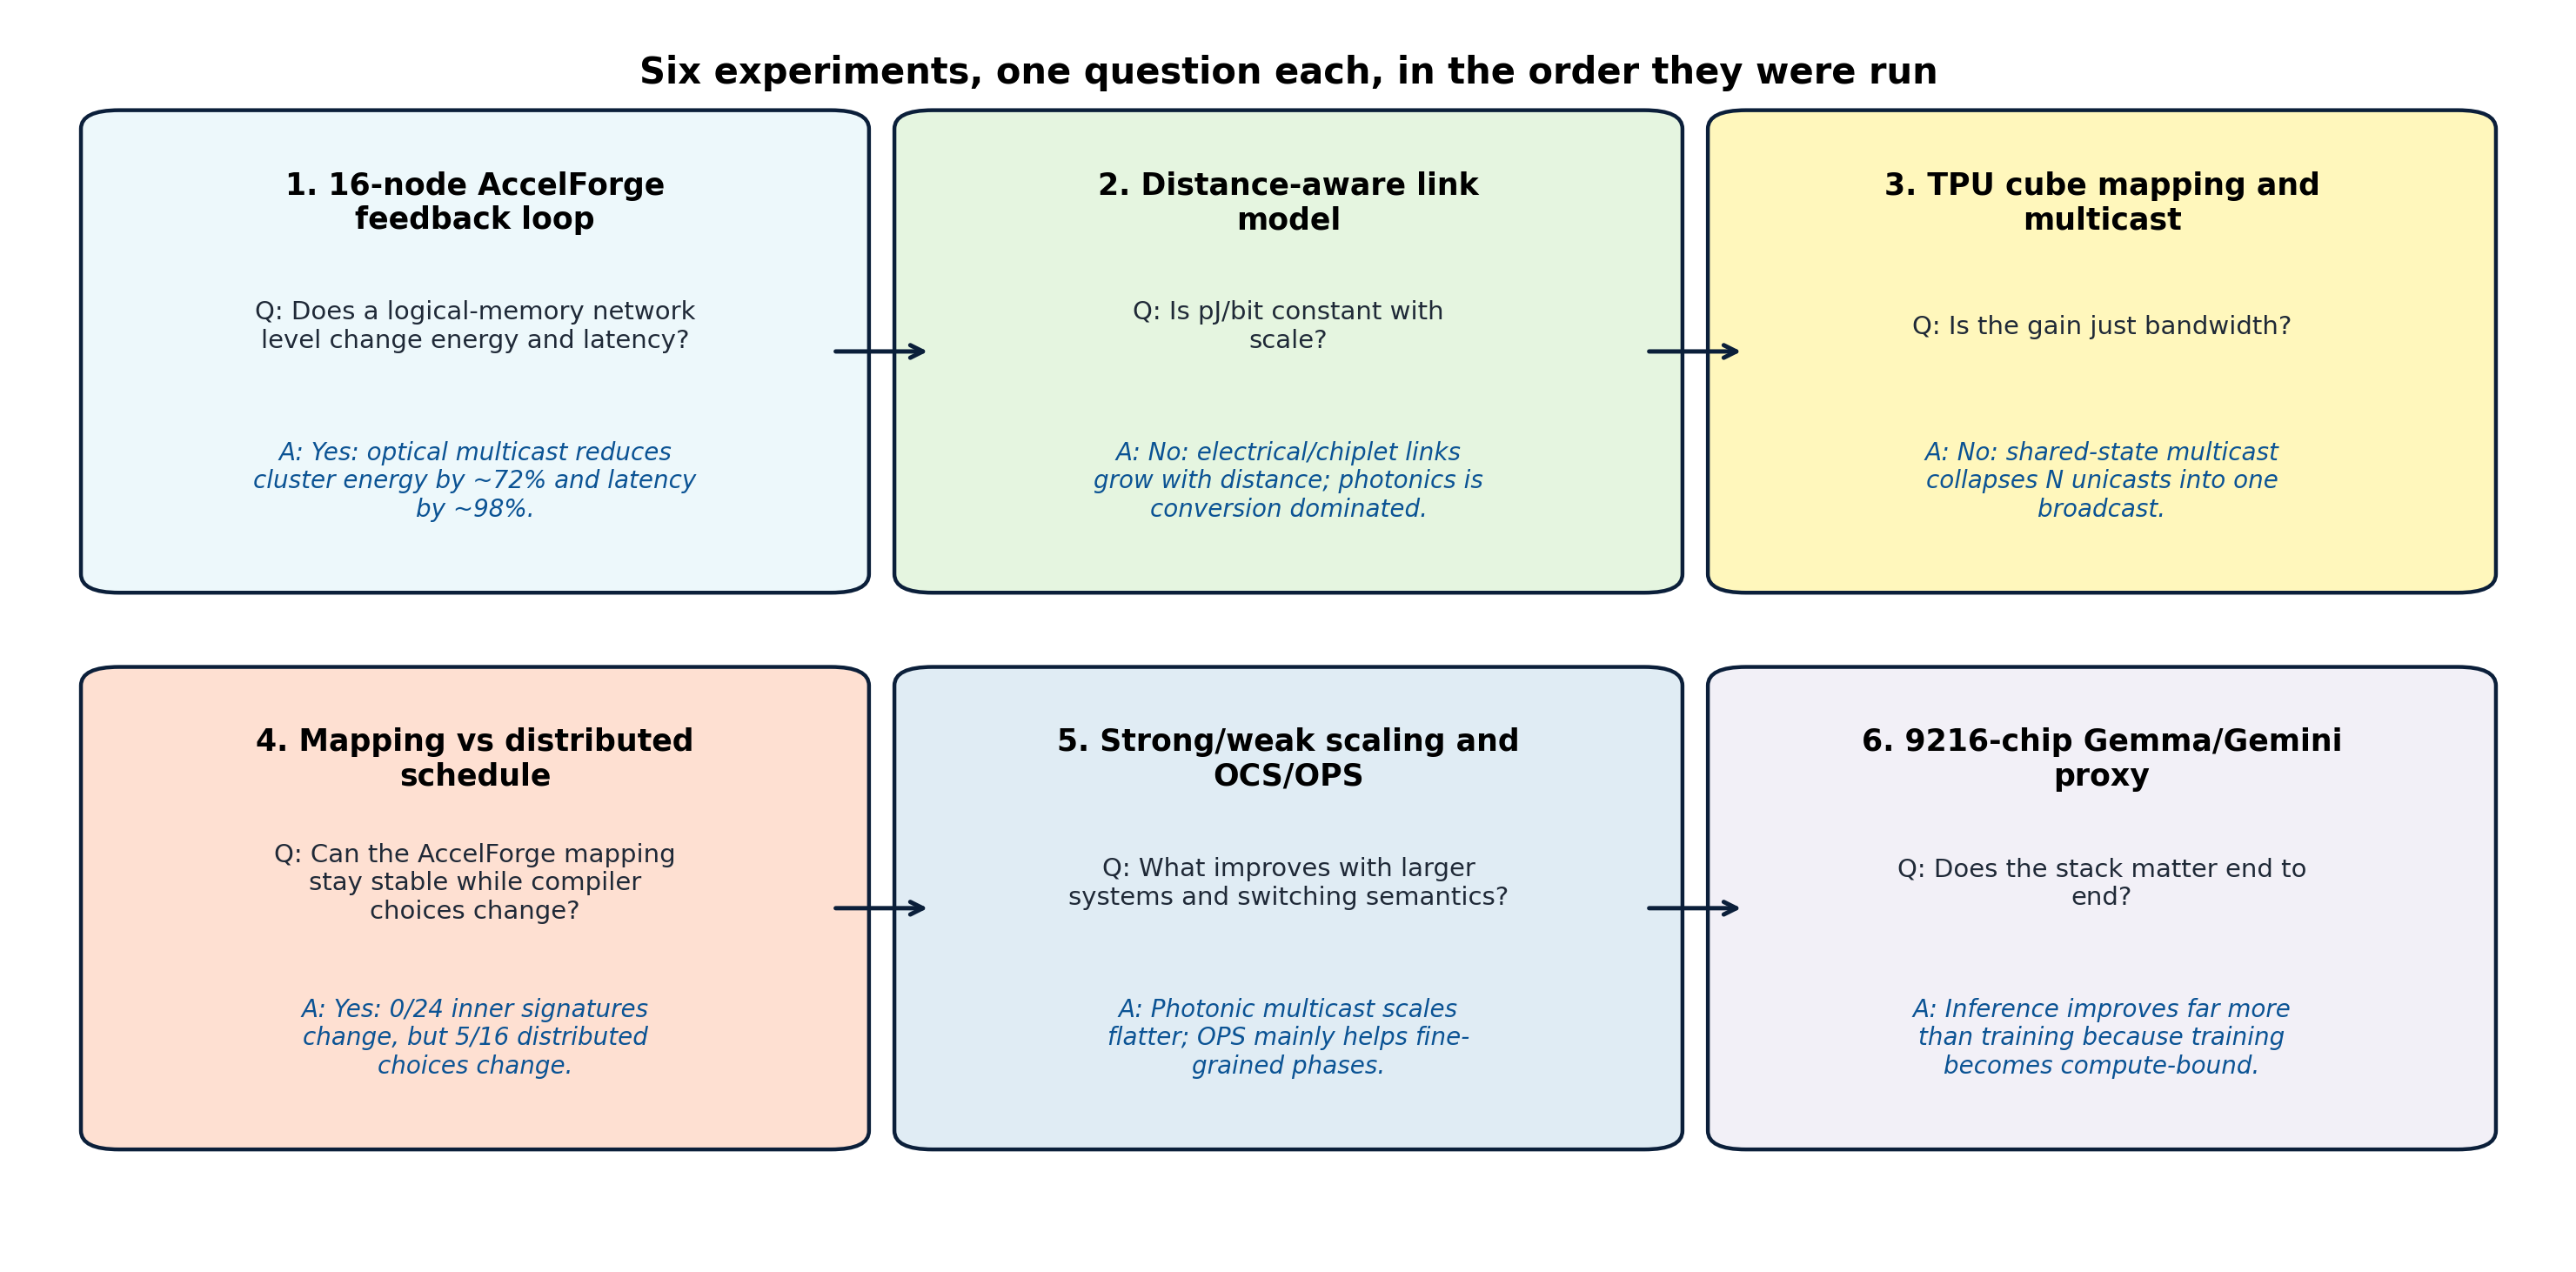
\includegraphics[width=\linewidth]{01_evidence_chain.png}
}
\end{columns}

\begin{columns}
\column{0.5}
\block{5. Results: Distance Physics and Mapping}{\centering
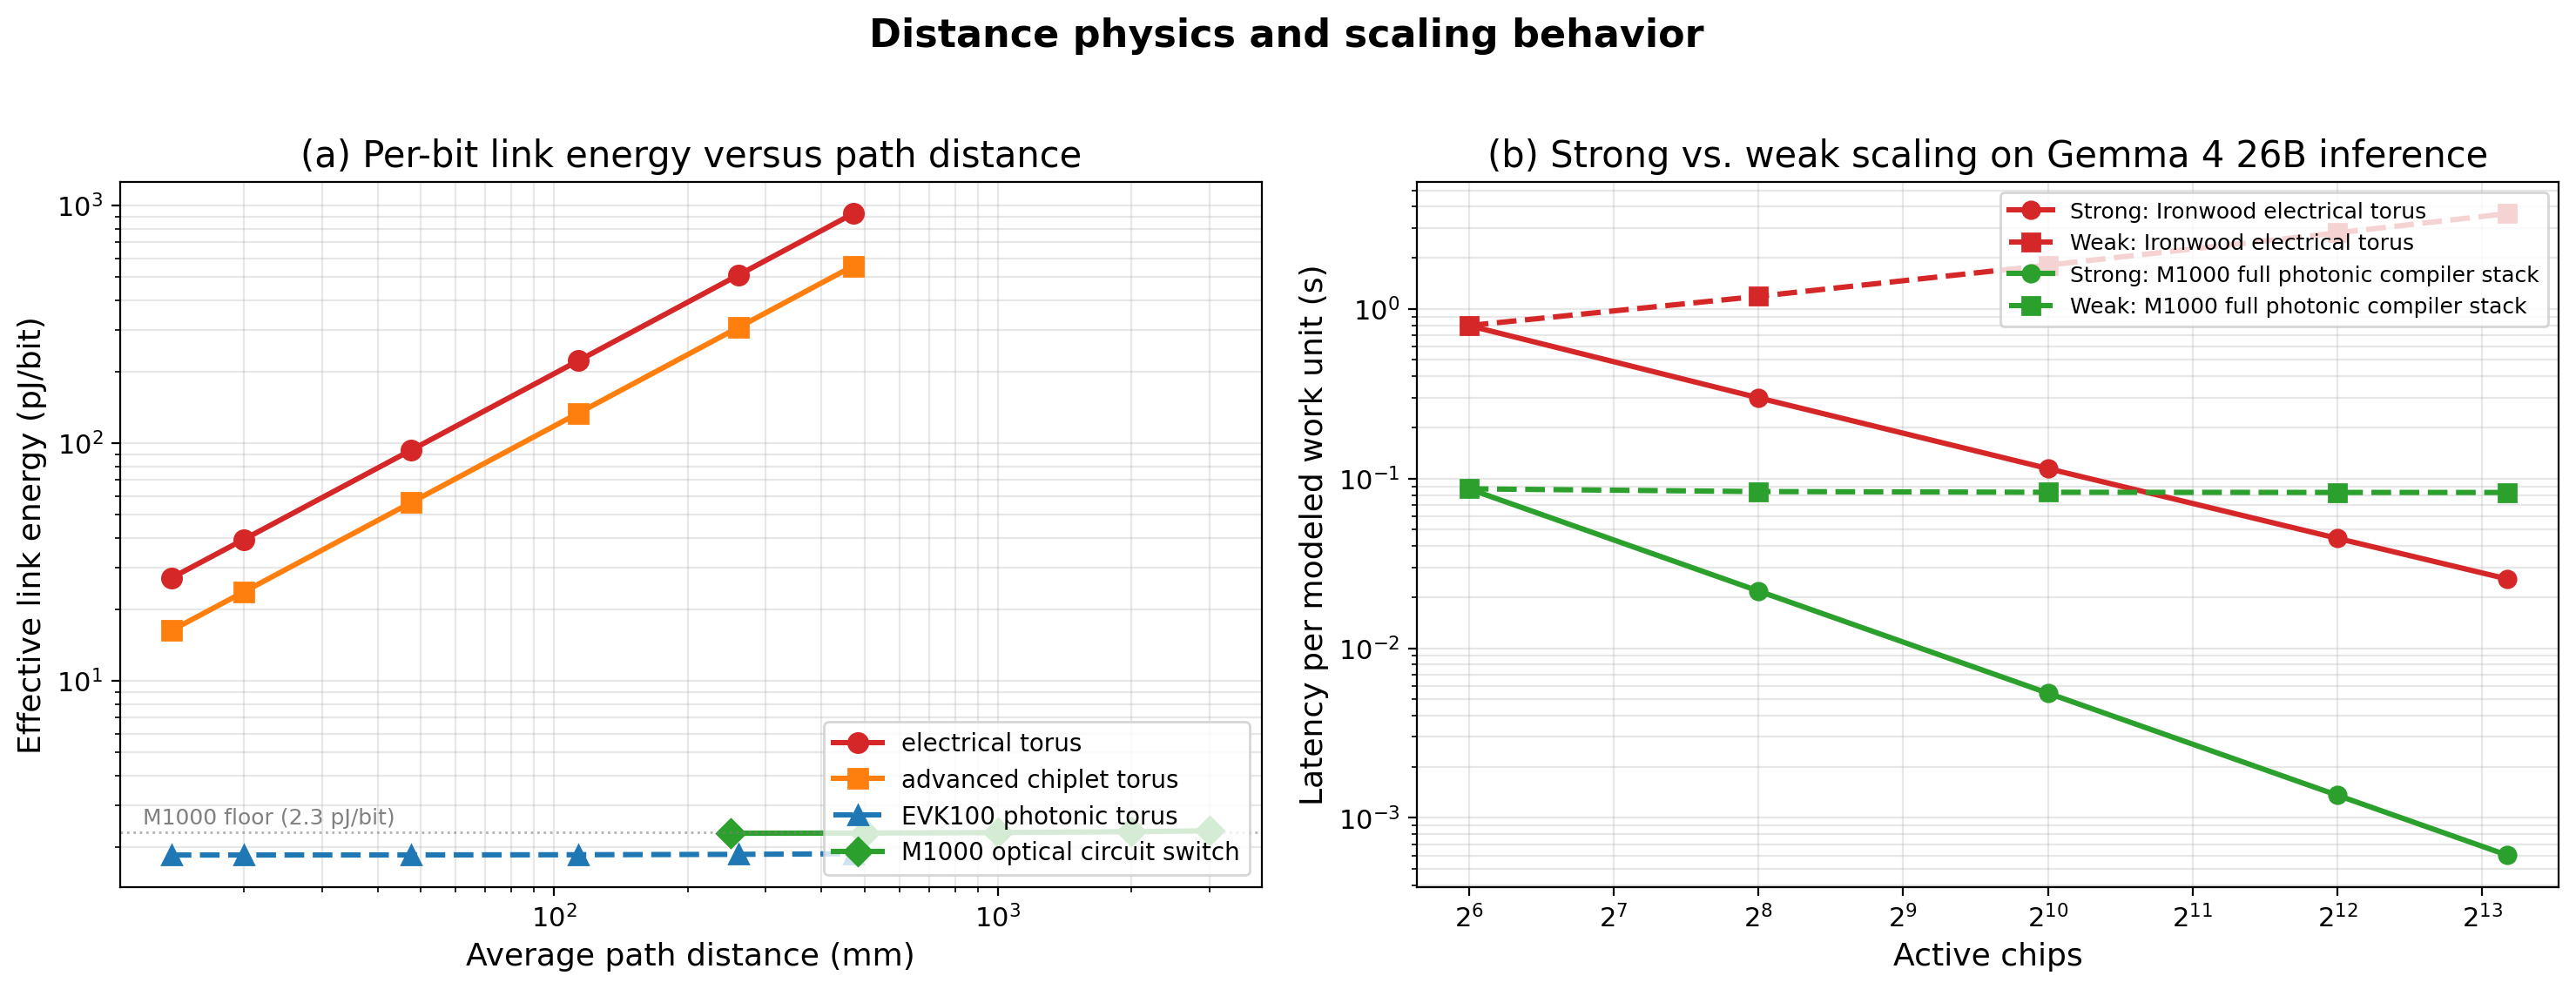
\includegraphics[width=\linewidth]{02_distance_and_scaling.png}\\[0.4em]
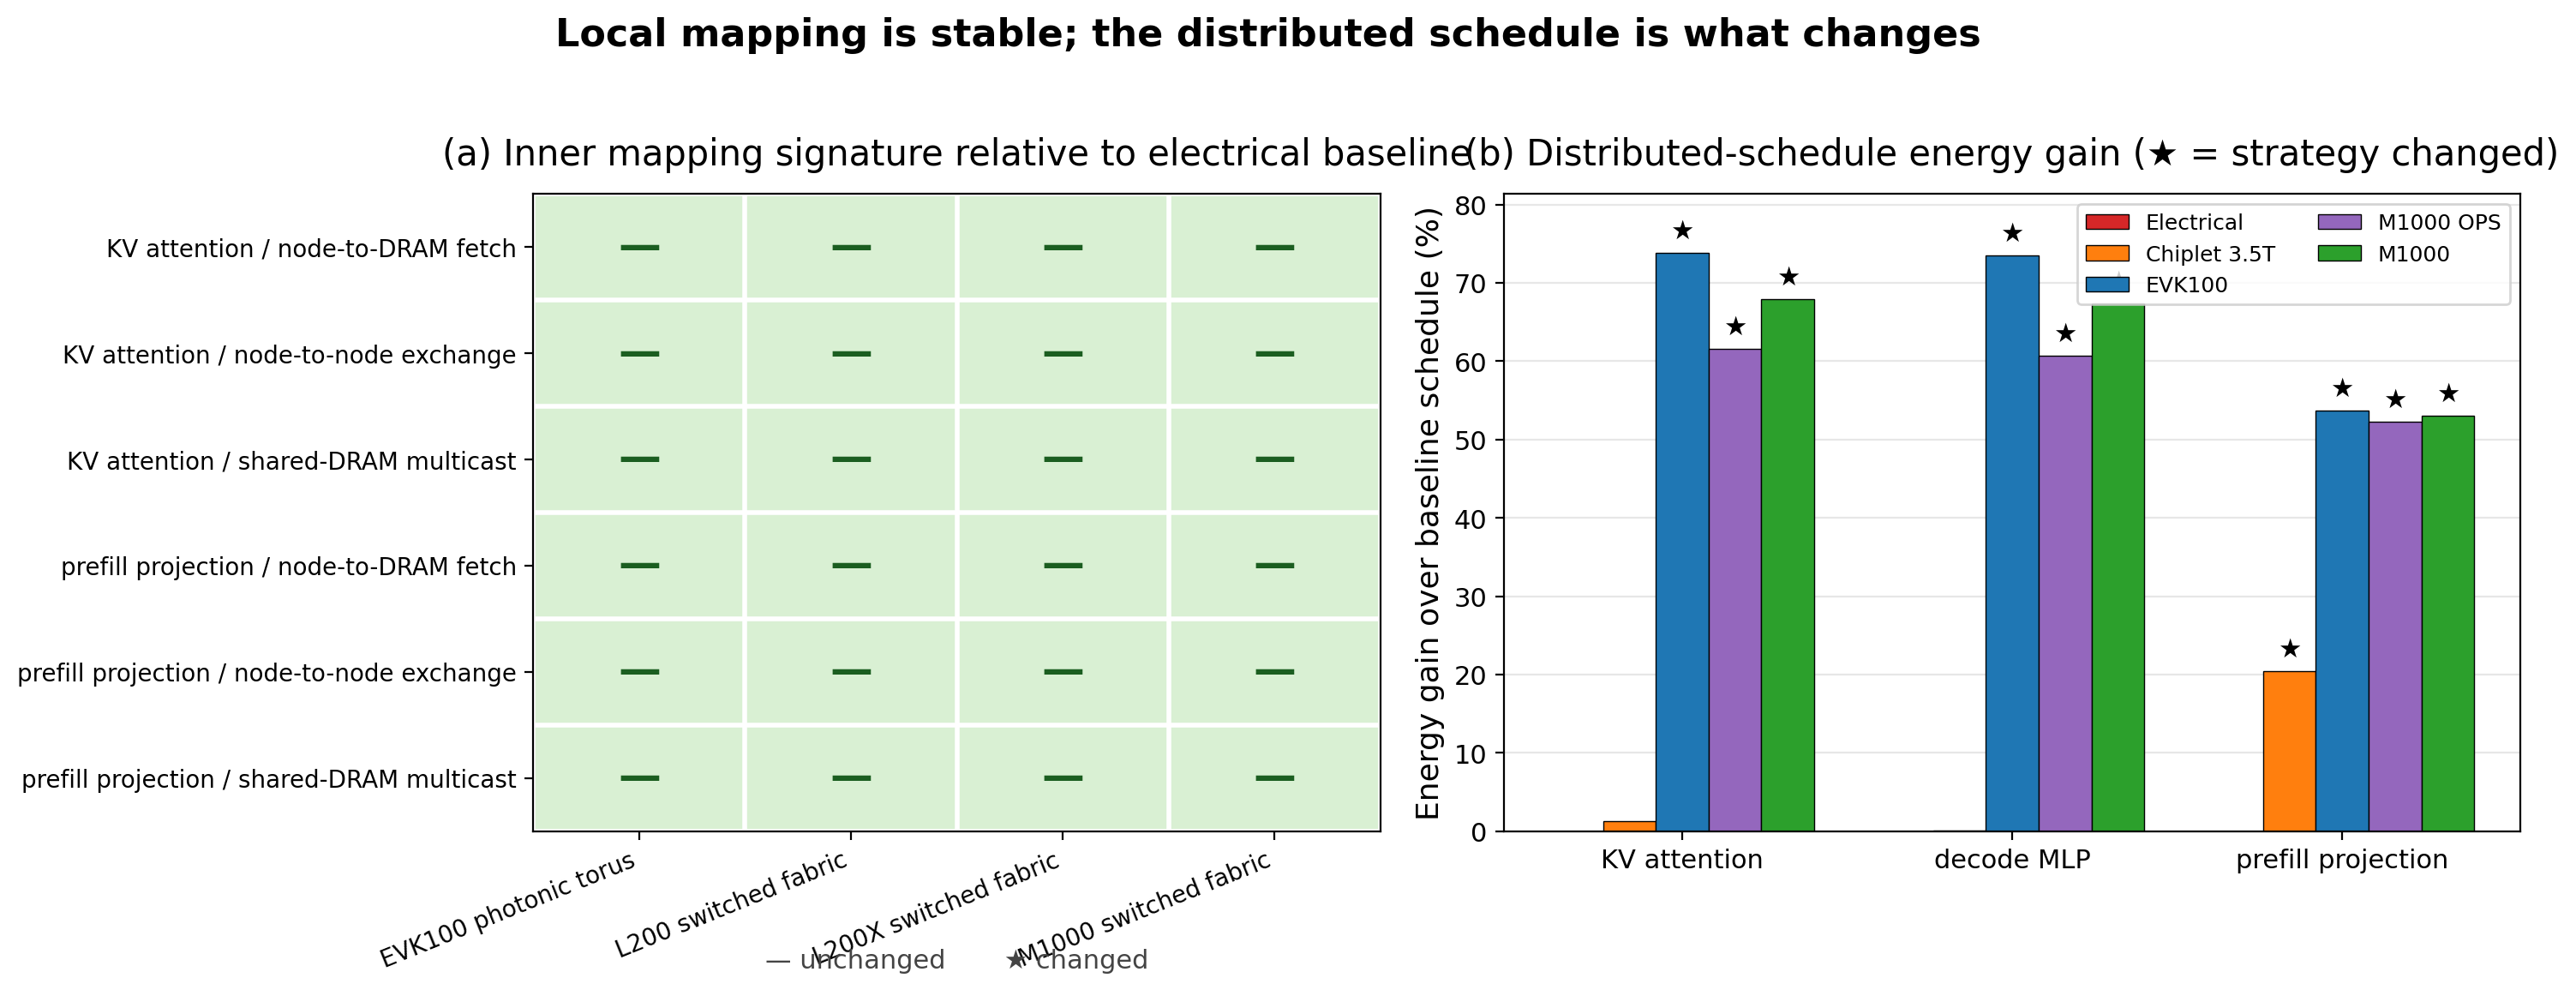
\includegraphics[width=\linewidth]{03_mapping_and_schedule.png}
}

\column{0.5}
\block{6. Results: Multicast and Pod Impact}{\centering
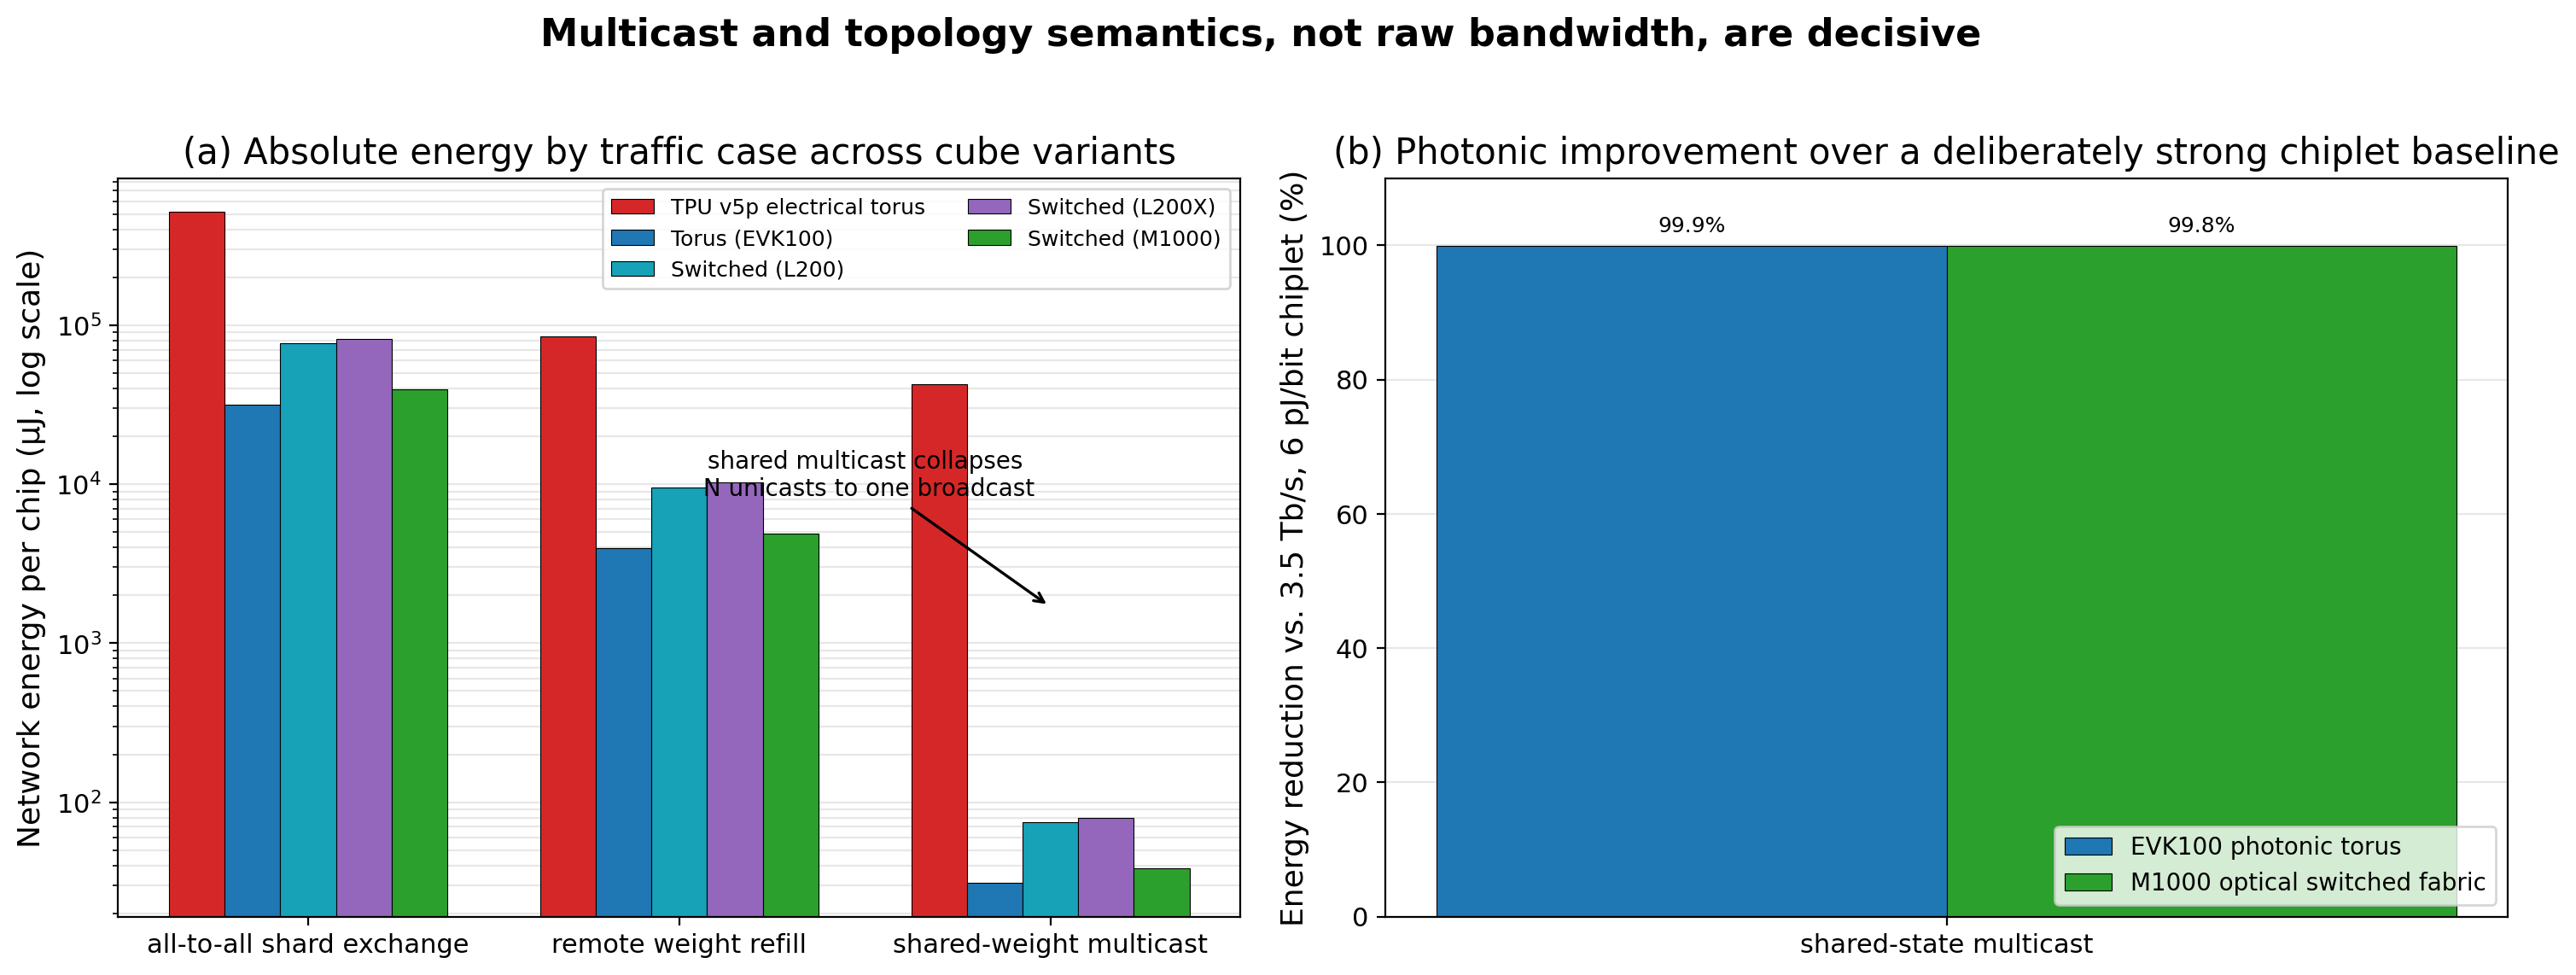
\includegraphics[width=\linewidth]{04_multicast_and_chiplet.png}\\[0.4em]
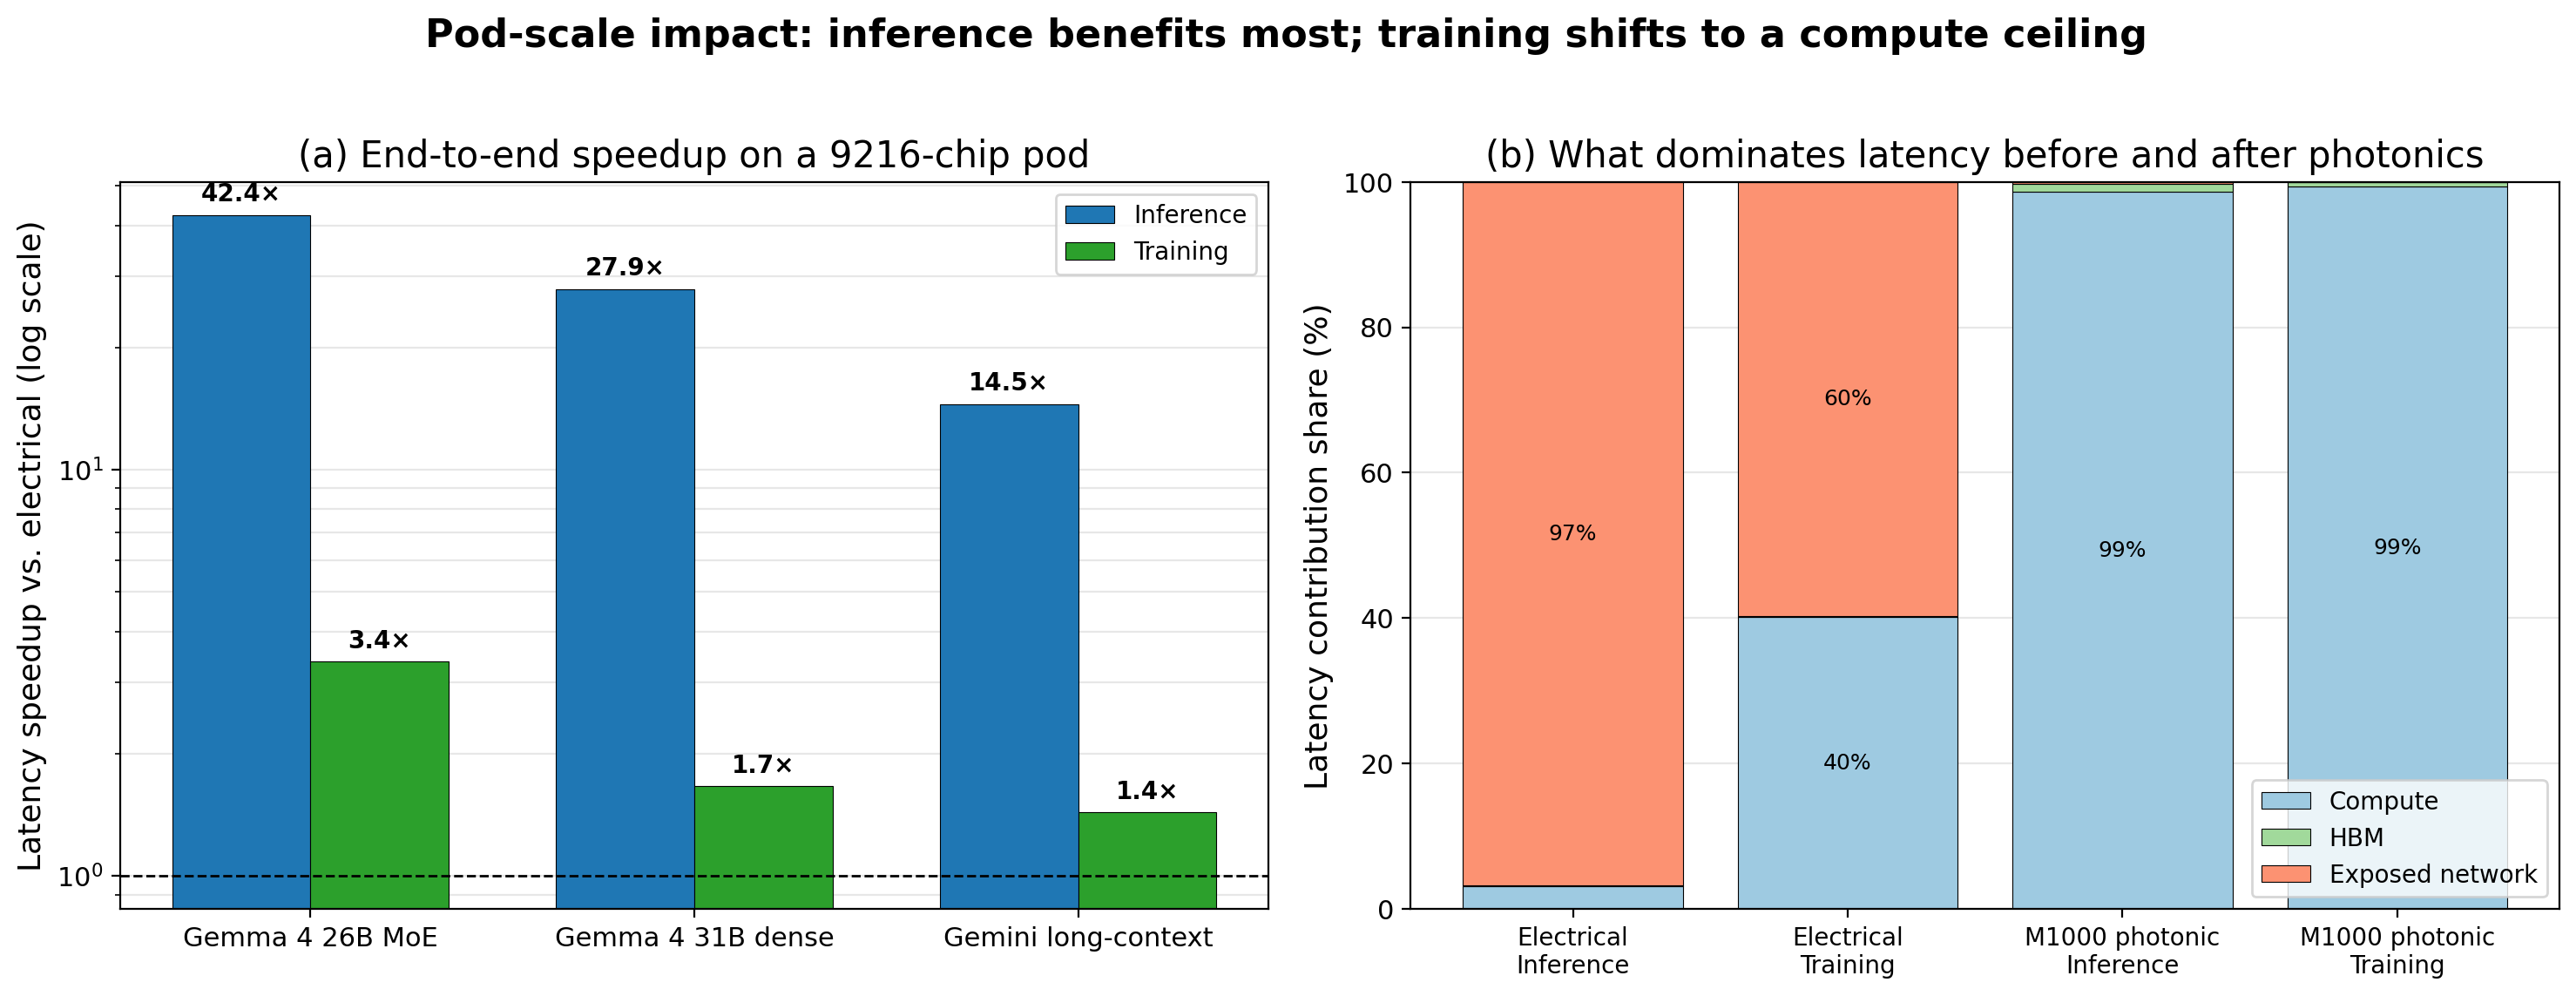
\includegraphics[width=\linewidth]{05_superpod_end_to_end.png}
}
\end{columns}

\begin{columns}
\column{0.5}
\block{7. Cluster Validation Heatmap}{\centering
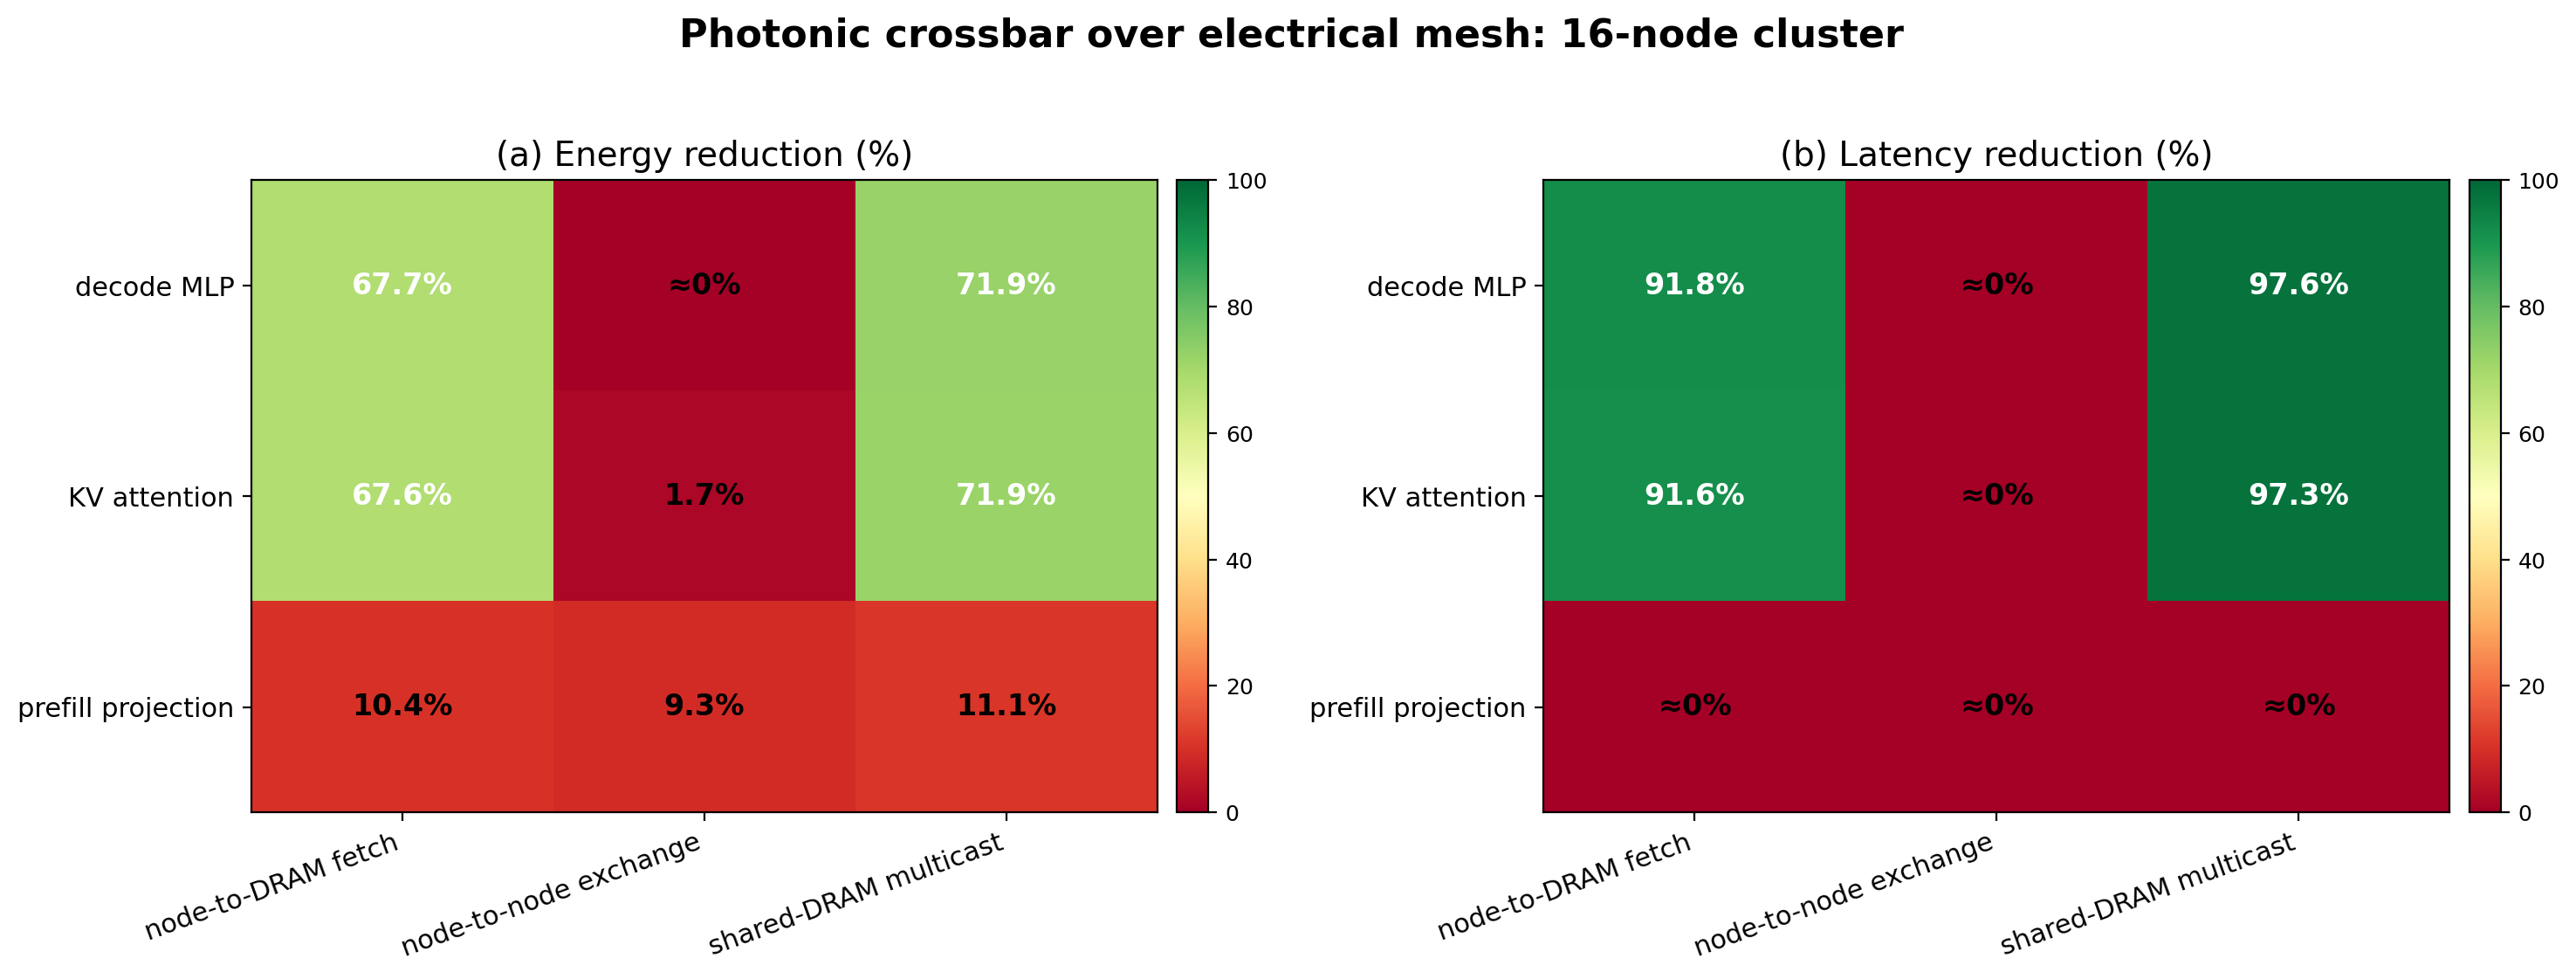
\includegraphics[width=\linewidth]{07_cluster_workload_heatmap.png}
}
\column{0.5}
\block{8. Switching and Residual Bottlenecks}{\centering
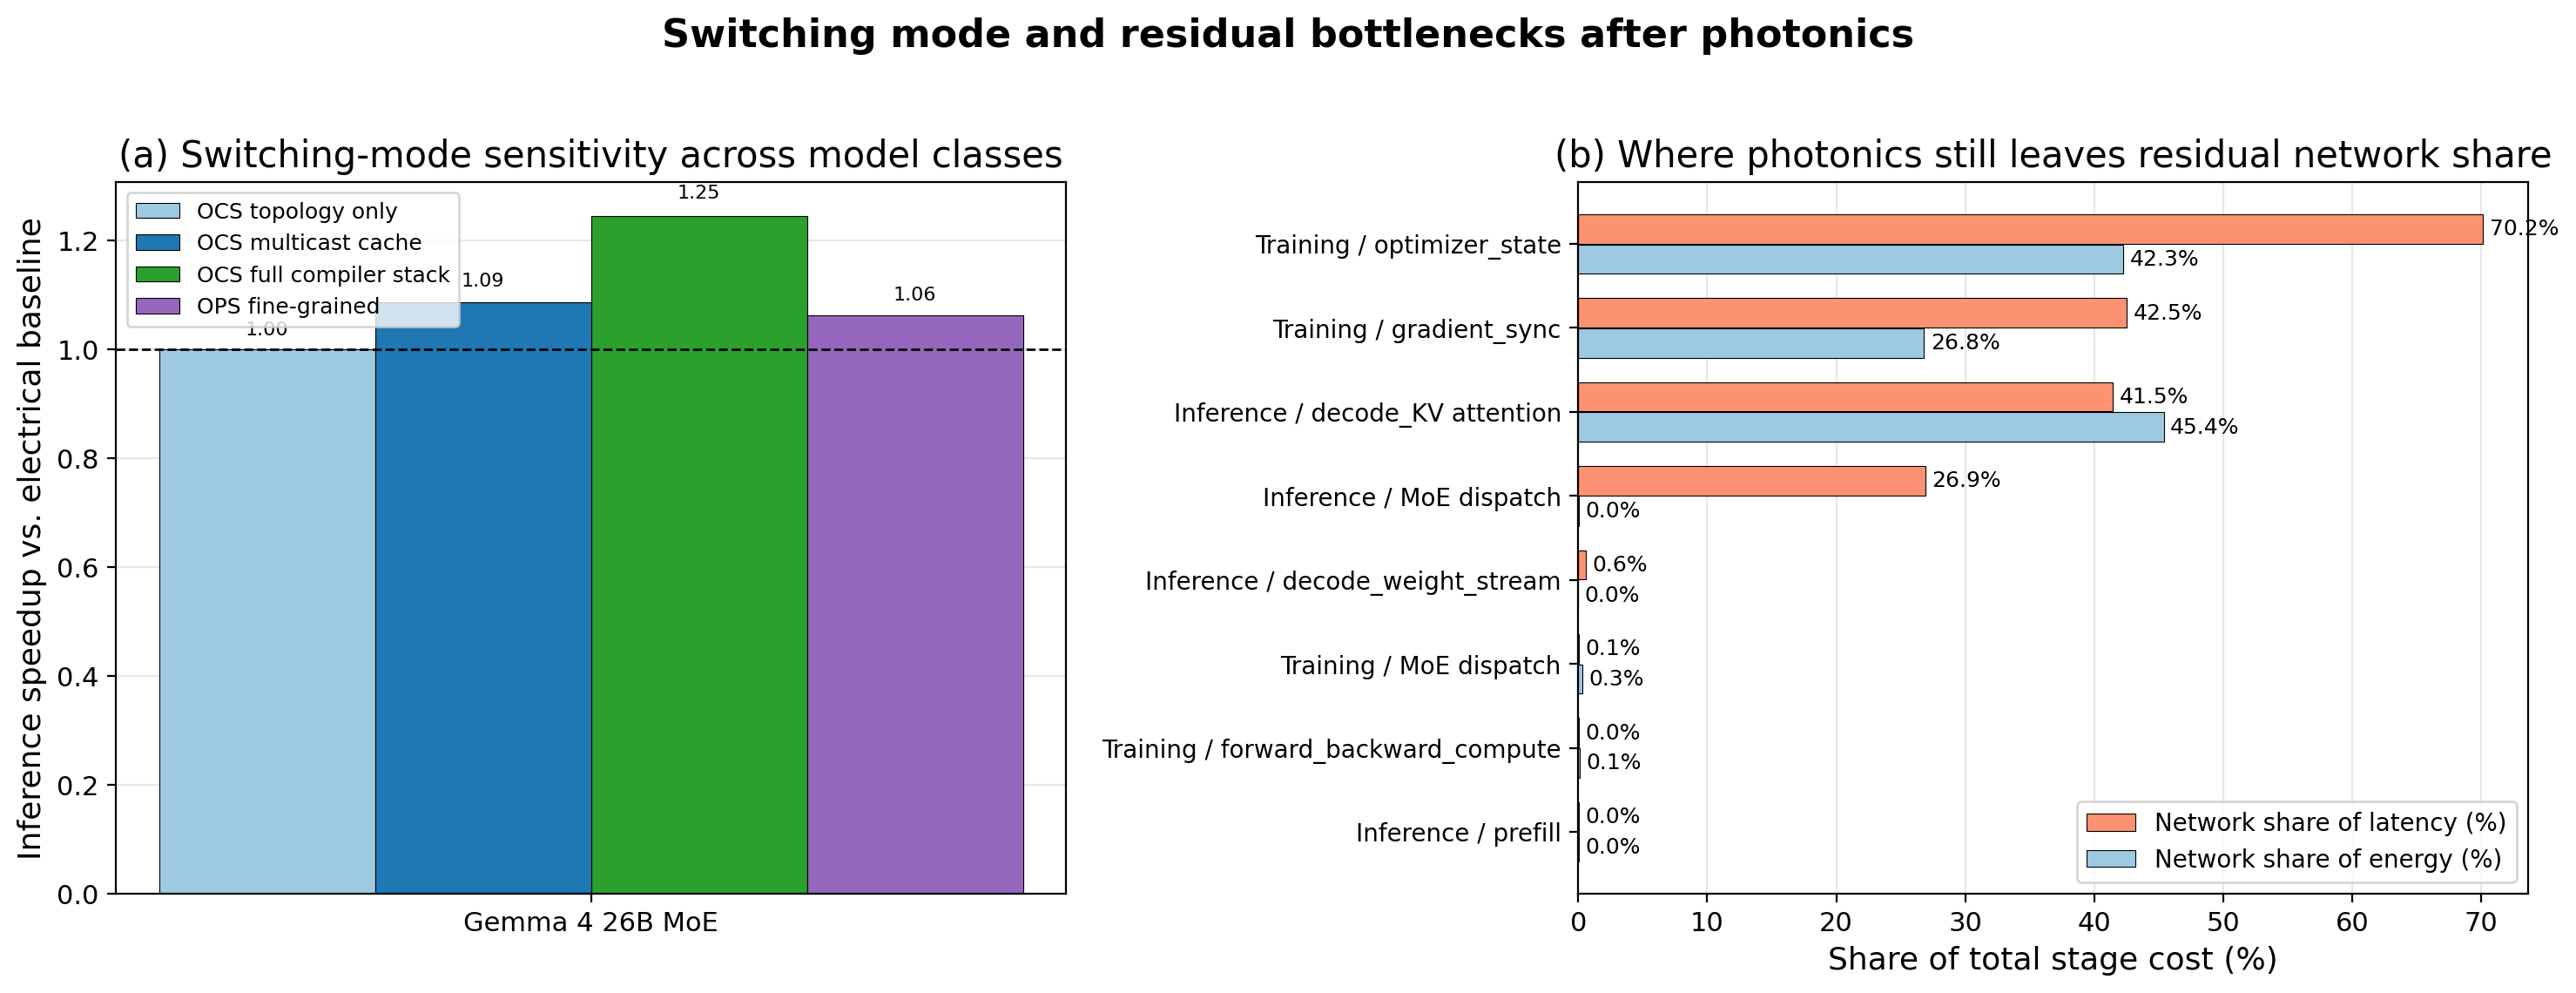
\includegraphics[width=\linewidth]{06_switching_and_limits.png}
}
\end{columns}

\block{9. Analysis of Results}{\normalsize
\begin{tabularx}{\linewidth}{lYY}
\toprule
Finding & Evidence & Interpretation \\
\midrule
Network-aware feedback changes system metrics & On a 16-node cluster the photonic crossbar reduces total energy by about 72\,\% and total latency by about 98\,\% on weight-dominated workloads & The logical-memory level is doing real work in the model, not just changing a label. \\
The local mapping does not move under the photonic swap & On the 64-chip torus, $0$ of $24$ inner mapping signatures differ from the electrical baseline across all photonic variants & Local GEMM dataflow is dominated by per-chip parameters, which we hold fixed. \\
The distributed schedule does change & $5$ of $16$ workload--architecture combinations switch from point-to-point exchange to shared multicast, and the best alternative schedule recovers up to 73.86\,\% of the original schedule's energy & The benefit lives one layer above the mapper, in compiler-visible territory. \\
Multicast, not raw bandwidth, is decisive & Even against a deliberately strong 3.5~\tbps{} 6~\pjbit{} chiplet baseline, photonic torus and switched fabrics reduce shared-multicast energy by close to 100\,\% & Topology semantics matter more than per-link bandwidth at pod scale. \\
Inference benefits much more than training & On a 9216-chip Ironwood-class pod, modeled inference latency improves about $42\times$ for the Gemma~4 MoE proxy while training improves about $3.4\times$ & Once communication shrinks, what remains is matrix-multiply compute. \\
\bottomrule
\end{tabularx}

\medskip
\textbf{What we do not claim.} The model deliberately excludes packet-level queueing, exact production compiler code generation, area and cost analysis, thermal drift, laser aging, and model-quality effects. Each of these is a follow-on study rather than a hidden assumption.
}

\block{References and Reproducibility}{\normalsize
Public sources include Google Cloud TPU7x and TPU v5p documentation; the Lightmatter Passage, Passage EVK100, and Passage M1000 EVK product pages; the PyTorch/XLA SPMD user guide; and recent course materials on einsums, mapping, memory hierarchies, and emerging accelerator technologies. The full chain of evidence in this poster is reproducible end-to-end from the project repository: every figure here is regenerated from a tabular evidence trail, and a regression suite locks in the central physics, multicast, mapping-invariance, and switching-mode claims.
}

\end{document}
